% \documentclass[dvipdfmx, 11pt]{beamer}
\documentclass[aspectratio=169, dvipdfmx, 11pt]{beamer} % aspectratio=43, 149, 169
\usepackage{here, amsmath, latexsym, amssymb, bm, ascmac, mathtools, multicol, tcolorbox, subfig}

% デザイン
\usetheme{Luebeck}
\usecolortheme{orchid}
\usefonttheme{professionalfonts}
\useinnertheme{circles}
\useoutertheme{infolines}
\setbeamercolor{title}{fg=structure, bg=}
\setbeamercolor{frametitle}{fg=structure, bg=}
\setbeamertemplate{itemize item}{\small\raise0.5pt\hbox{$\bullet$}}
\setbeamertemplate{itemize subitem}{\tiny\raise1.5pt\hbox{$\blacktriangleright$}}
\setbeamertemplate{itemize subsubitem}{\tiny\raise1.5pt\hbox{$\bigstar$}}

%しおりの文字化け解消
\usepackage{atbegshi}
\ifnum 42146=\euc"A4A2
\AtBeginShipoutFirst{\special{pdf:tounicode EUC-UCS2}}
\else
\AtBeginShipoutFirst{\special{pdf:tounicode 90ms-RKSJ-UCS2}}
\fi

\setbeamertemplate{navigation symbols}{}
\renewcommand{\kanjifamilydefault}{\gtdefault}
\newcommand{\red}[1]{\textcolor{red}{#1}}
\newcommand{\green}[1]{\textcolor{green!40!black}{#1}}
\newcommand{\blue}[1]{\textcolor{blue!80!black}{#1}}

\title[Day01]{機械学習の基礎}
\subtitle{Day01}
\author[Yudai Fujimoto]{Yudai Fujimoto}
\institute[SUS]{Suwa University of Science}
\date{\today}

\begin{document}
\maketitle

\begin{frame}{目次}
    \tableofcontents
\end{frame}

\section{機械学習の概要}
\begin{frame}{機械学習とは}
    機械学習とは、コンピューターがデータを分析する手法の1つで「ML(Machine Learning)」とも呼ばれています。
    大量のデータを学習する際に、一定のルールやパターンを見つけ出し、次回同じような課題に直面した際に以前学習した
    ルールやパターンを用いることでより良い予測や判断をすることができます。
\end{frame}

\begin{frame}{機械学習の流れ}
    機械学習には学習、推論と呼ばれる2つのステップが存在する。
    \begin{block}{1.学習}
    学習用(train data)データから特徴などを読み取り、正しい推論が行えるように、パラメータを更新していく(モデルを賢くする)こと。
    \end{block}
    \begin{alertblock}{2.推論(inference)}
    学習が完了したモデルを用いて機械学習で問題を解くこと。 \\
    例: 回帰、分類、物体検出、自然言語処理、時系列情報予測
    \end{alertblock}
\end{frame}

\begin{frame}{3種類の機械学習}
    機械学習には大まかに3つの種類に分類できる。
    \begin{block}{教師あり学習}
    ラベル付けされたデータを用いる。
    \end{block}
    \begin{alertblock}{教師なし学習}
    データのみからデータの隠れた法則を見つけ出す。
    \end{alertblock}
    \begin{exampleblock}{強化学習}
    最も良い環境のやり取りを見つけ出す。
    \end{exampleblock}
\end{frame}

\begin{frame}{教師あり学習}
    3つある機械学習の手法の中で最も代表出来な手法。 \\
    主な目的は、ラベル付けされた訓練データををもとにモデルを学習し、
    ラベル付けされていないのデータをもデータに対して、正しい予測を行うとこ。\\
    主なタスク
    \begin{itemize}
        \item 分類: どのクラスに属しているかを予測する(画像分類など)
        \item 回帰: どのような値になるかを予測する(株価予測など)
    \end{itemize}
    \begin{figure}[b]
        \begin{center}
        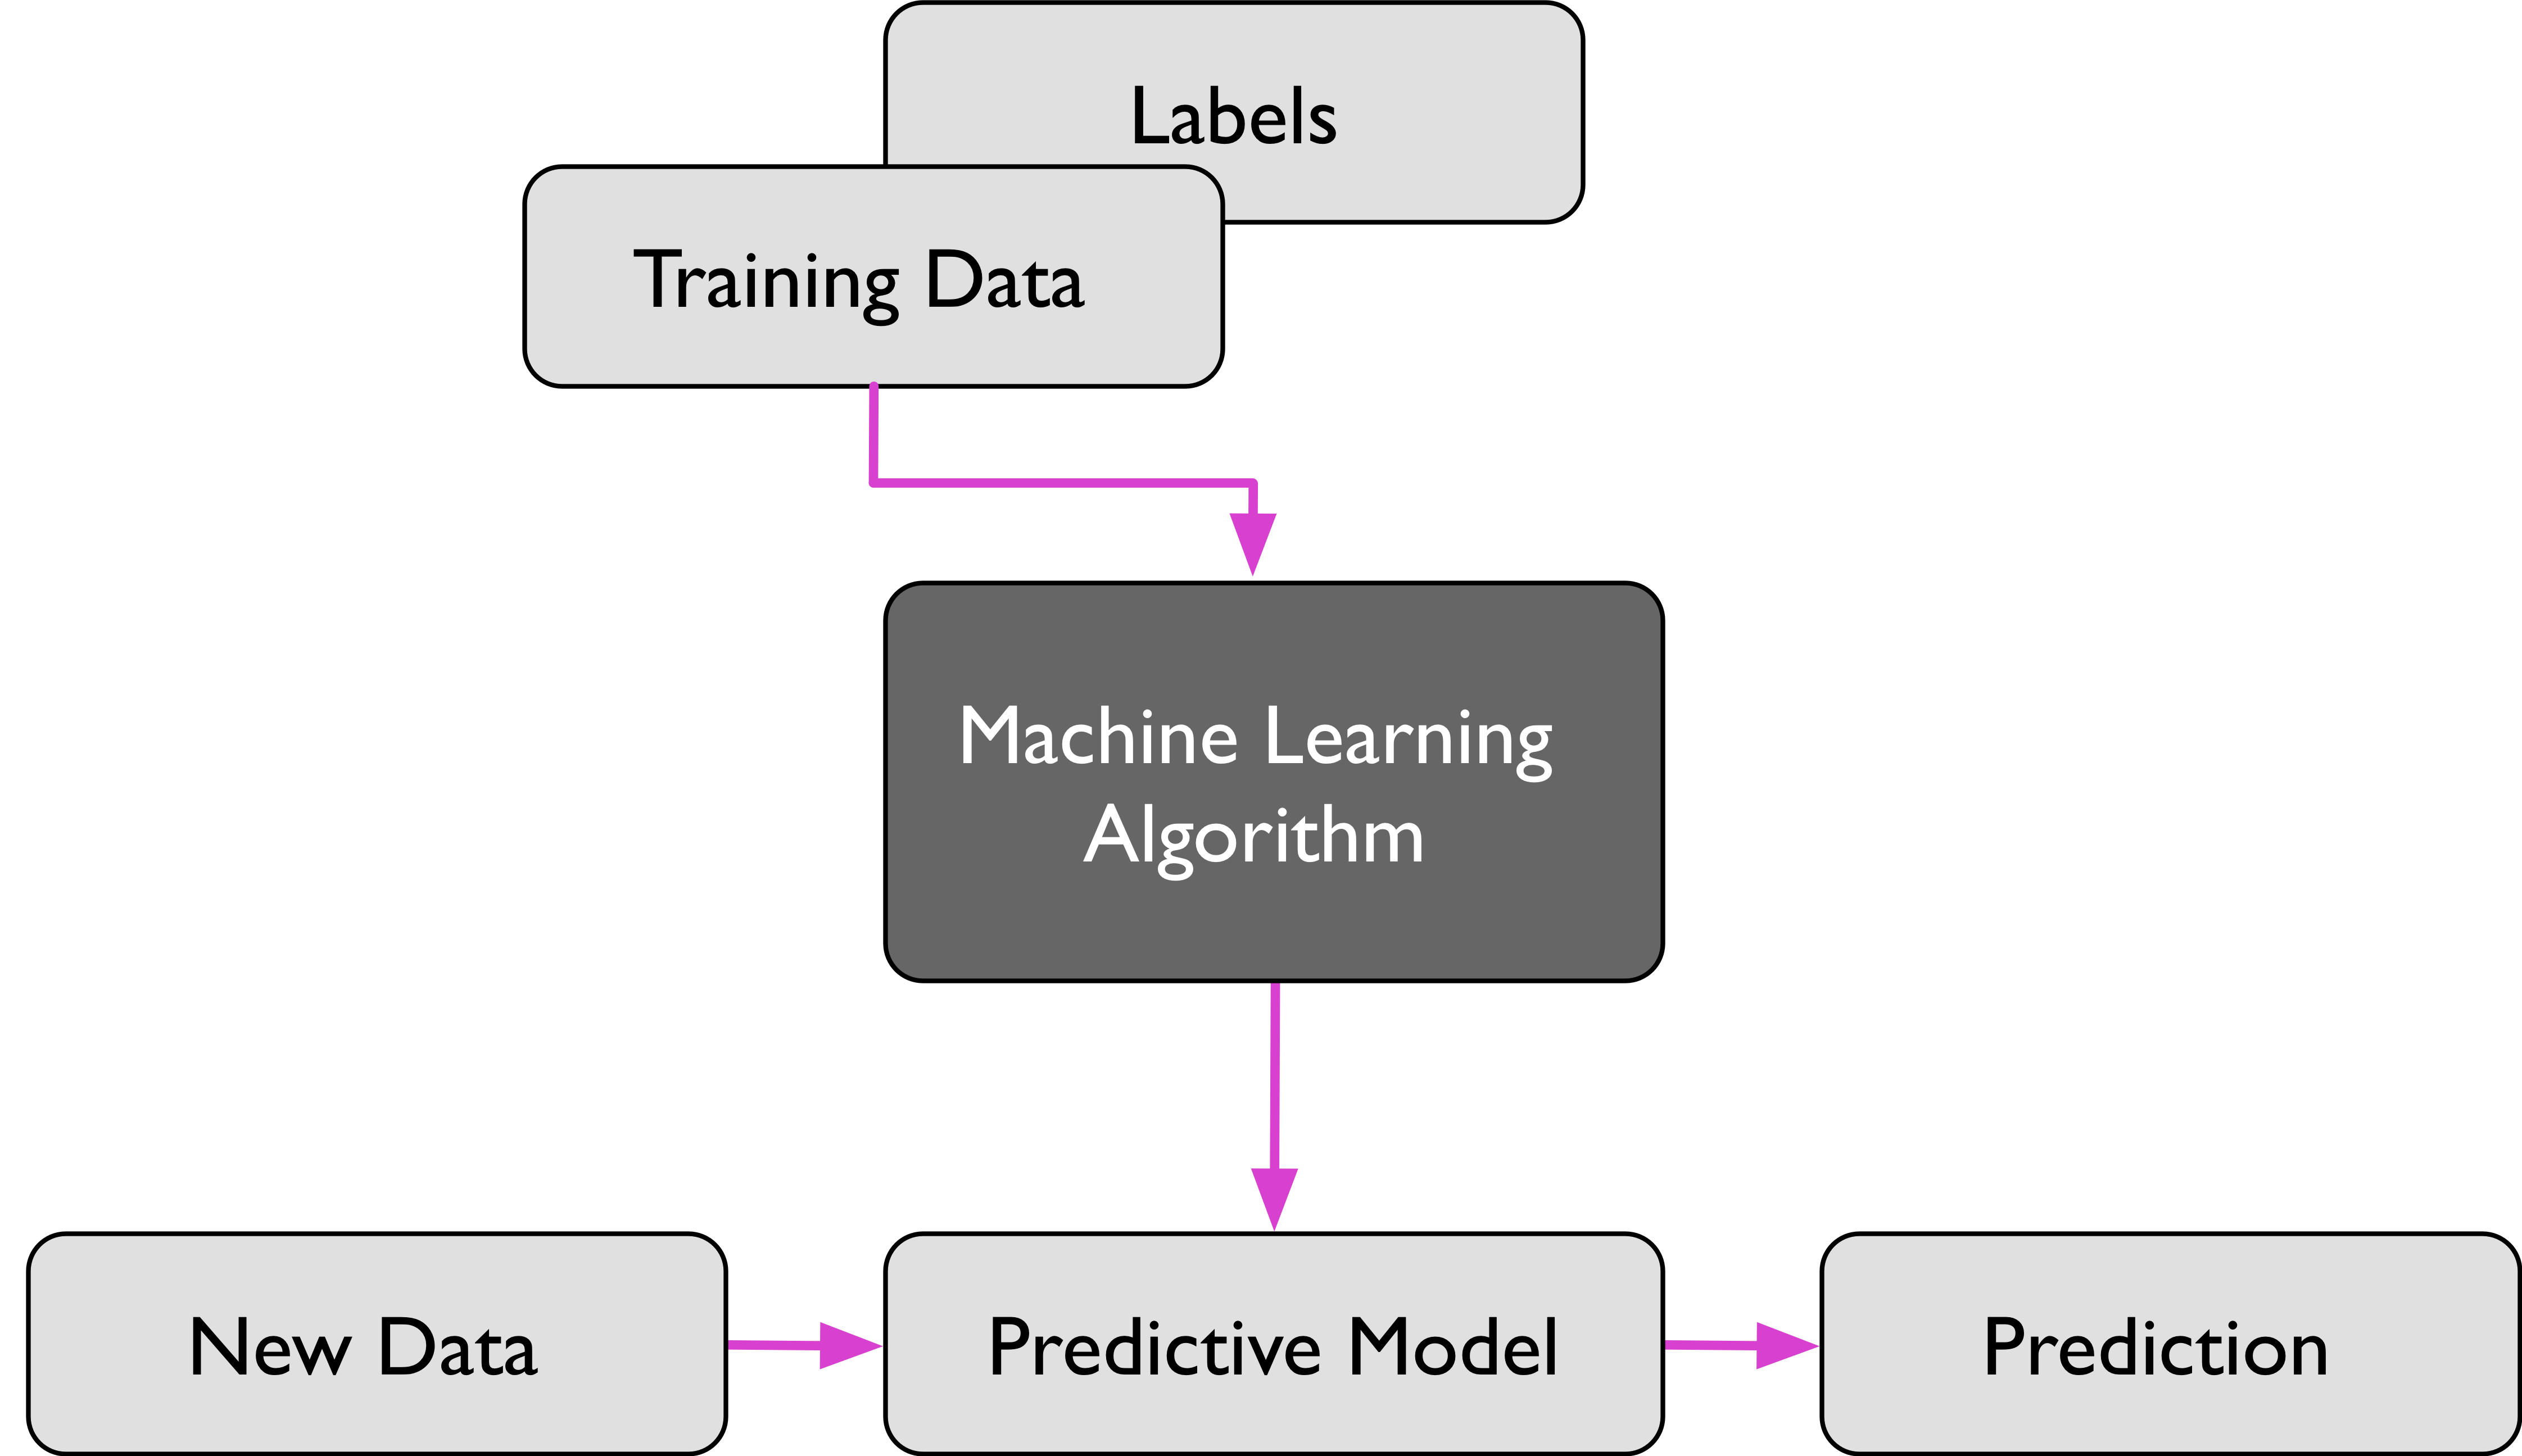
\includegraphics[width=60mm]{img/day01/fig01.png}
        \end{center}
    \end{figure}        
\end{frame}

\begin{frame}{教師なし学習}
教師なし学習は、学習データに正解データを与えない状態で学習させる学習手法です。 \\
教師データが与えられないので、データのみからデータの隠れた特徴を見つけ出します。 \\
主なタスク
\begin{itemize}
    \item クラスリング: データをグループ分けする
    \item 次元削減: 次元削減はデータを特徴づける情報を抽出し、データの次元数を減らす
\end{itemize}
\begin{figure}[h]
    \begin{minipage}[b]{0.45\linewidth}
        \centering
        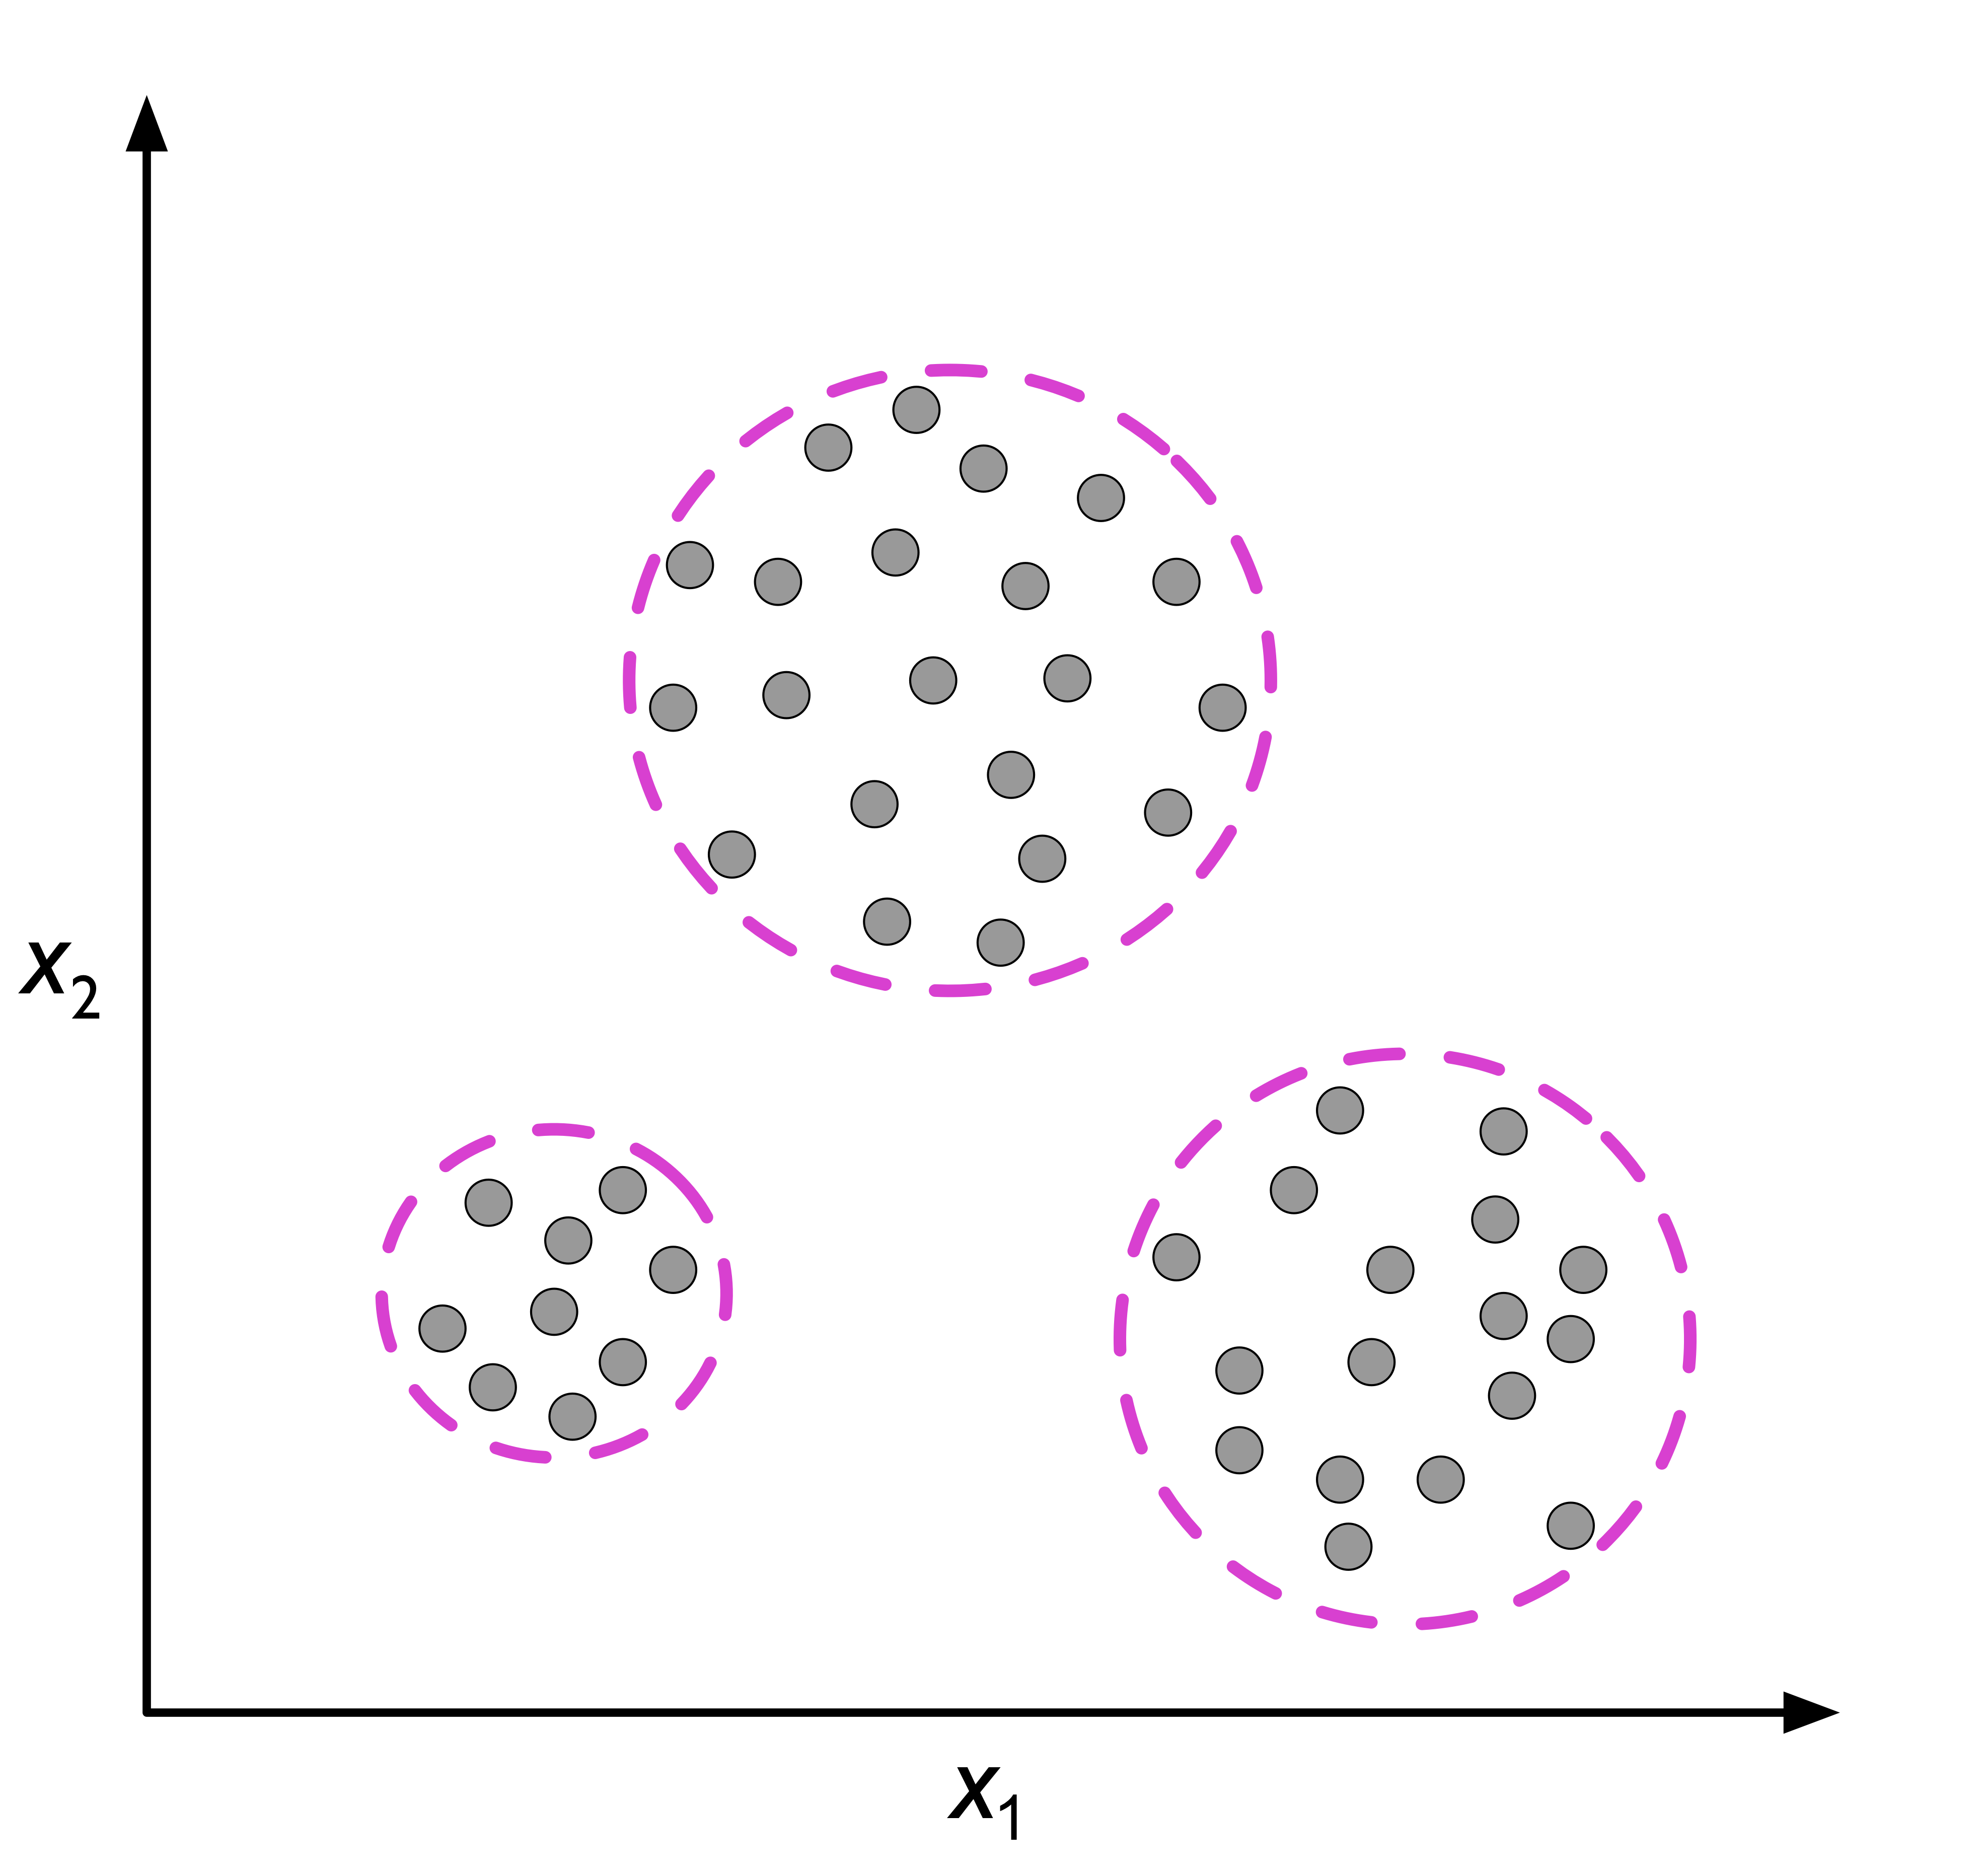
\includegraphics[width=30mm]{img/day01/fig02.png}
        \caption*{クラスタリング}
    \end{minipage}
    \begin{minipage}[b]{0.45\linewidth}
        \centering
        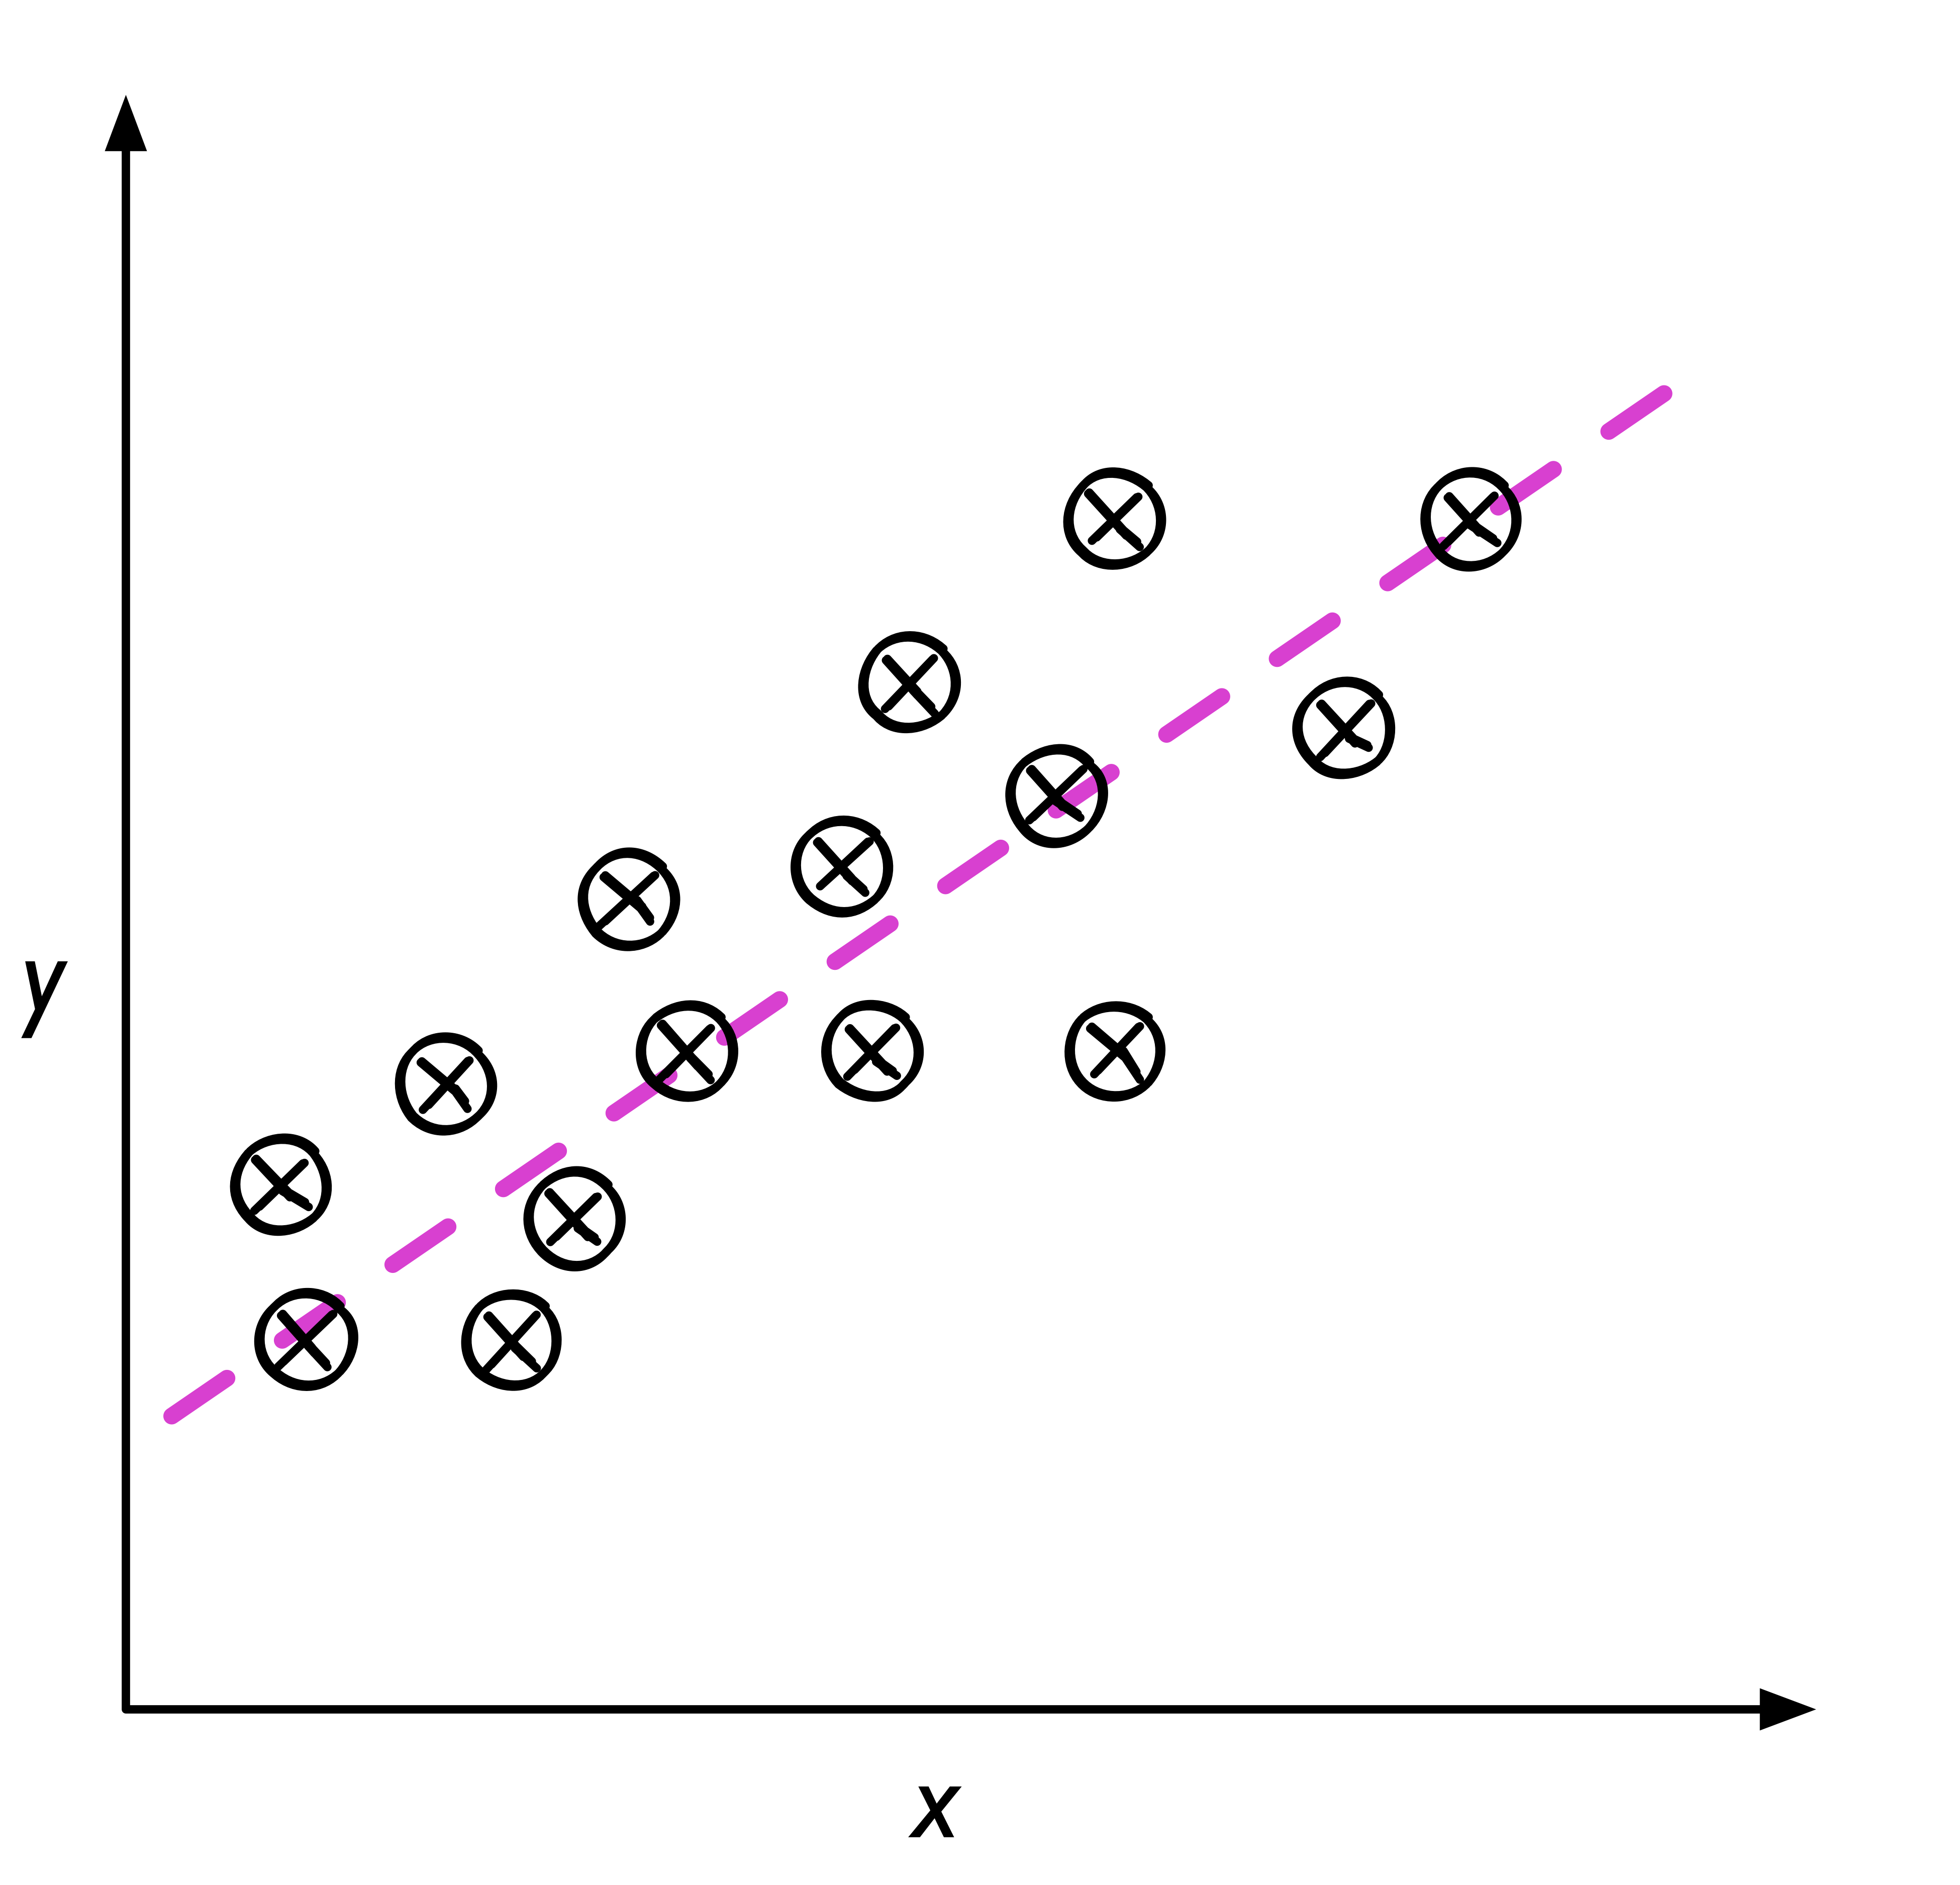
\includegraphics[width=30mm]{img/day01/fig03.png}
        \caption*{次元削減}
    \end{minipage}
\end{figure}
\end{frame}

\begin{frame}{強化学習}
    教師として正解のデータがあるわけではなく、与えられるのは試行錯誤をする中で「良かったか悪かったか」という情報(Reward)のみ。
    RewardもとにどのようなActionをすべきなのかを学習をする手法。 \\
    主なタスク
    \begin{itemize}
        \item AIプレイヤー(AlphaGoなど)
        \item AIによる振動抑制
    \end{itemize}
    \begin{figure}[b]
        \begin{center}
        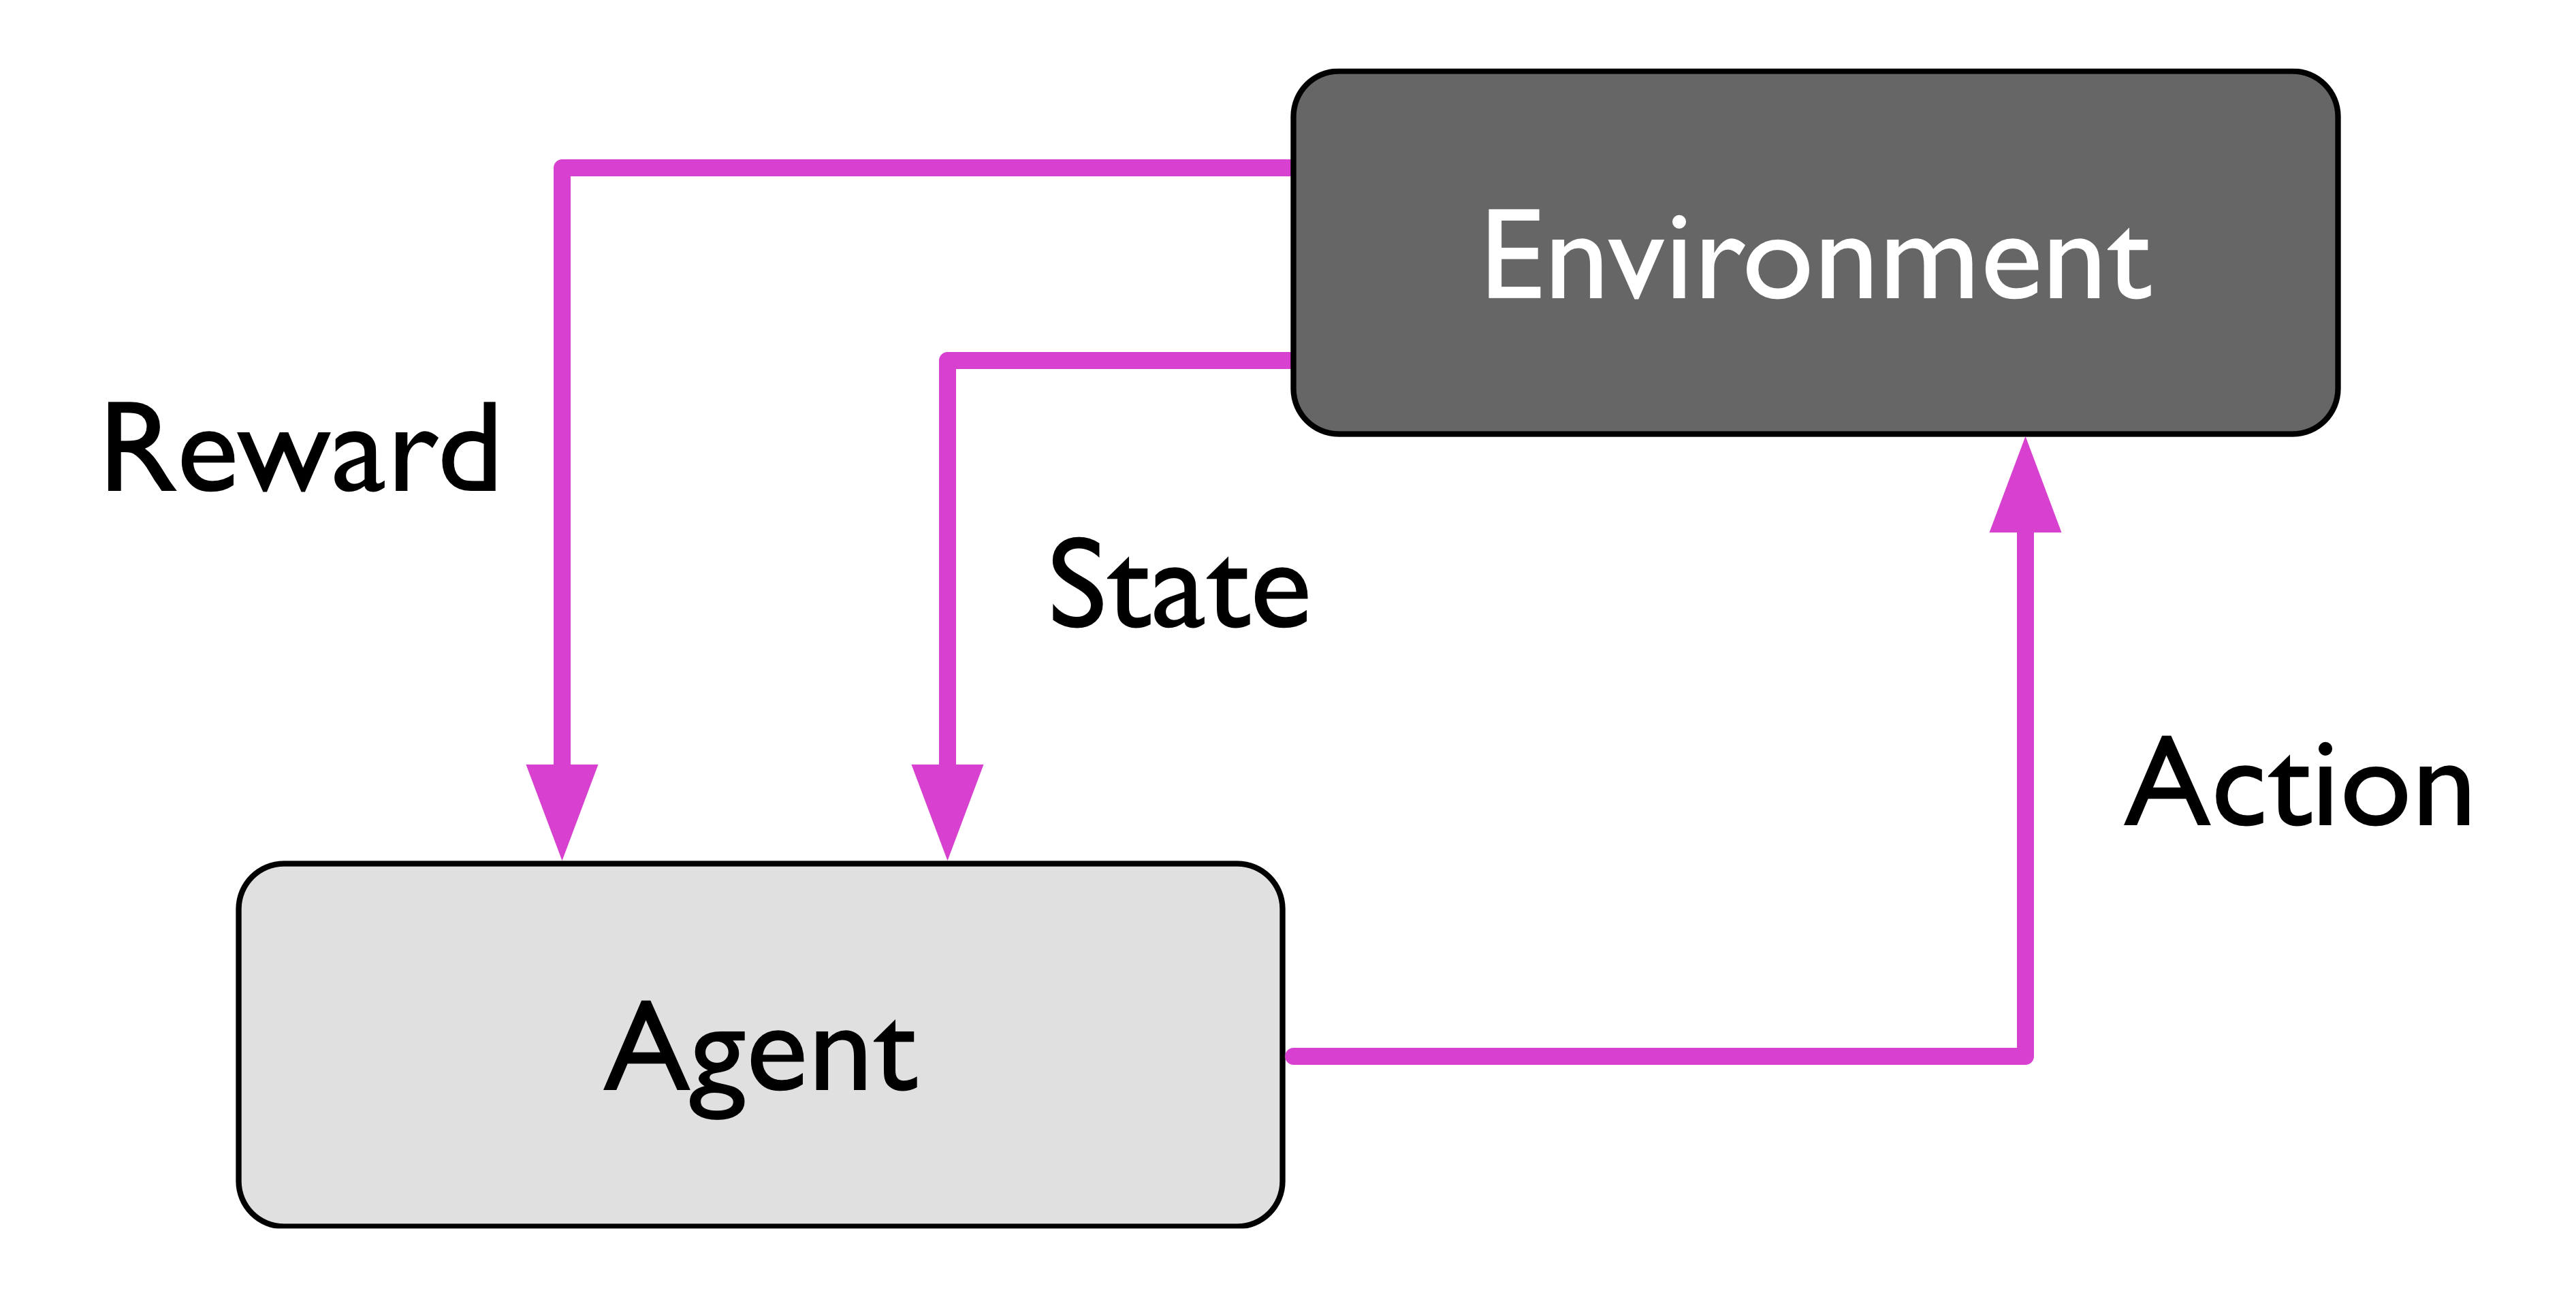
\includegraphics[width=60mm]{img/day01/fig04.png}
        \end{center}
    \end{figure}  
\end{frame}

\section{教師あり学習にチャレンジ}
\begin{frame}{教師あり学習にチャレンジ}
    ヤマメの花のデータセット(Iris Dataset)を用いてどのヤマメなのかを推測するタスク。
    \begin{itemize}
        \item 特徴量: 花びら(Petal)の長さ/幅, がく片(Septal)の長さ/幅
        \item ラベル: ヤマメの種類(Setosa/Versicolor/Virginica)
    \end{itemize}
    \begin{figure}[h]
        \begin{center}
        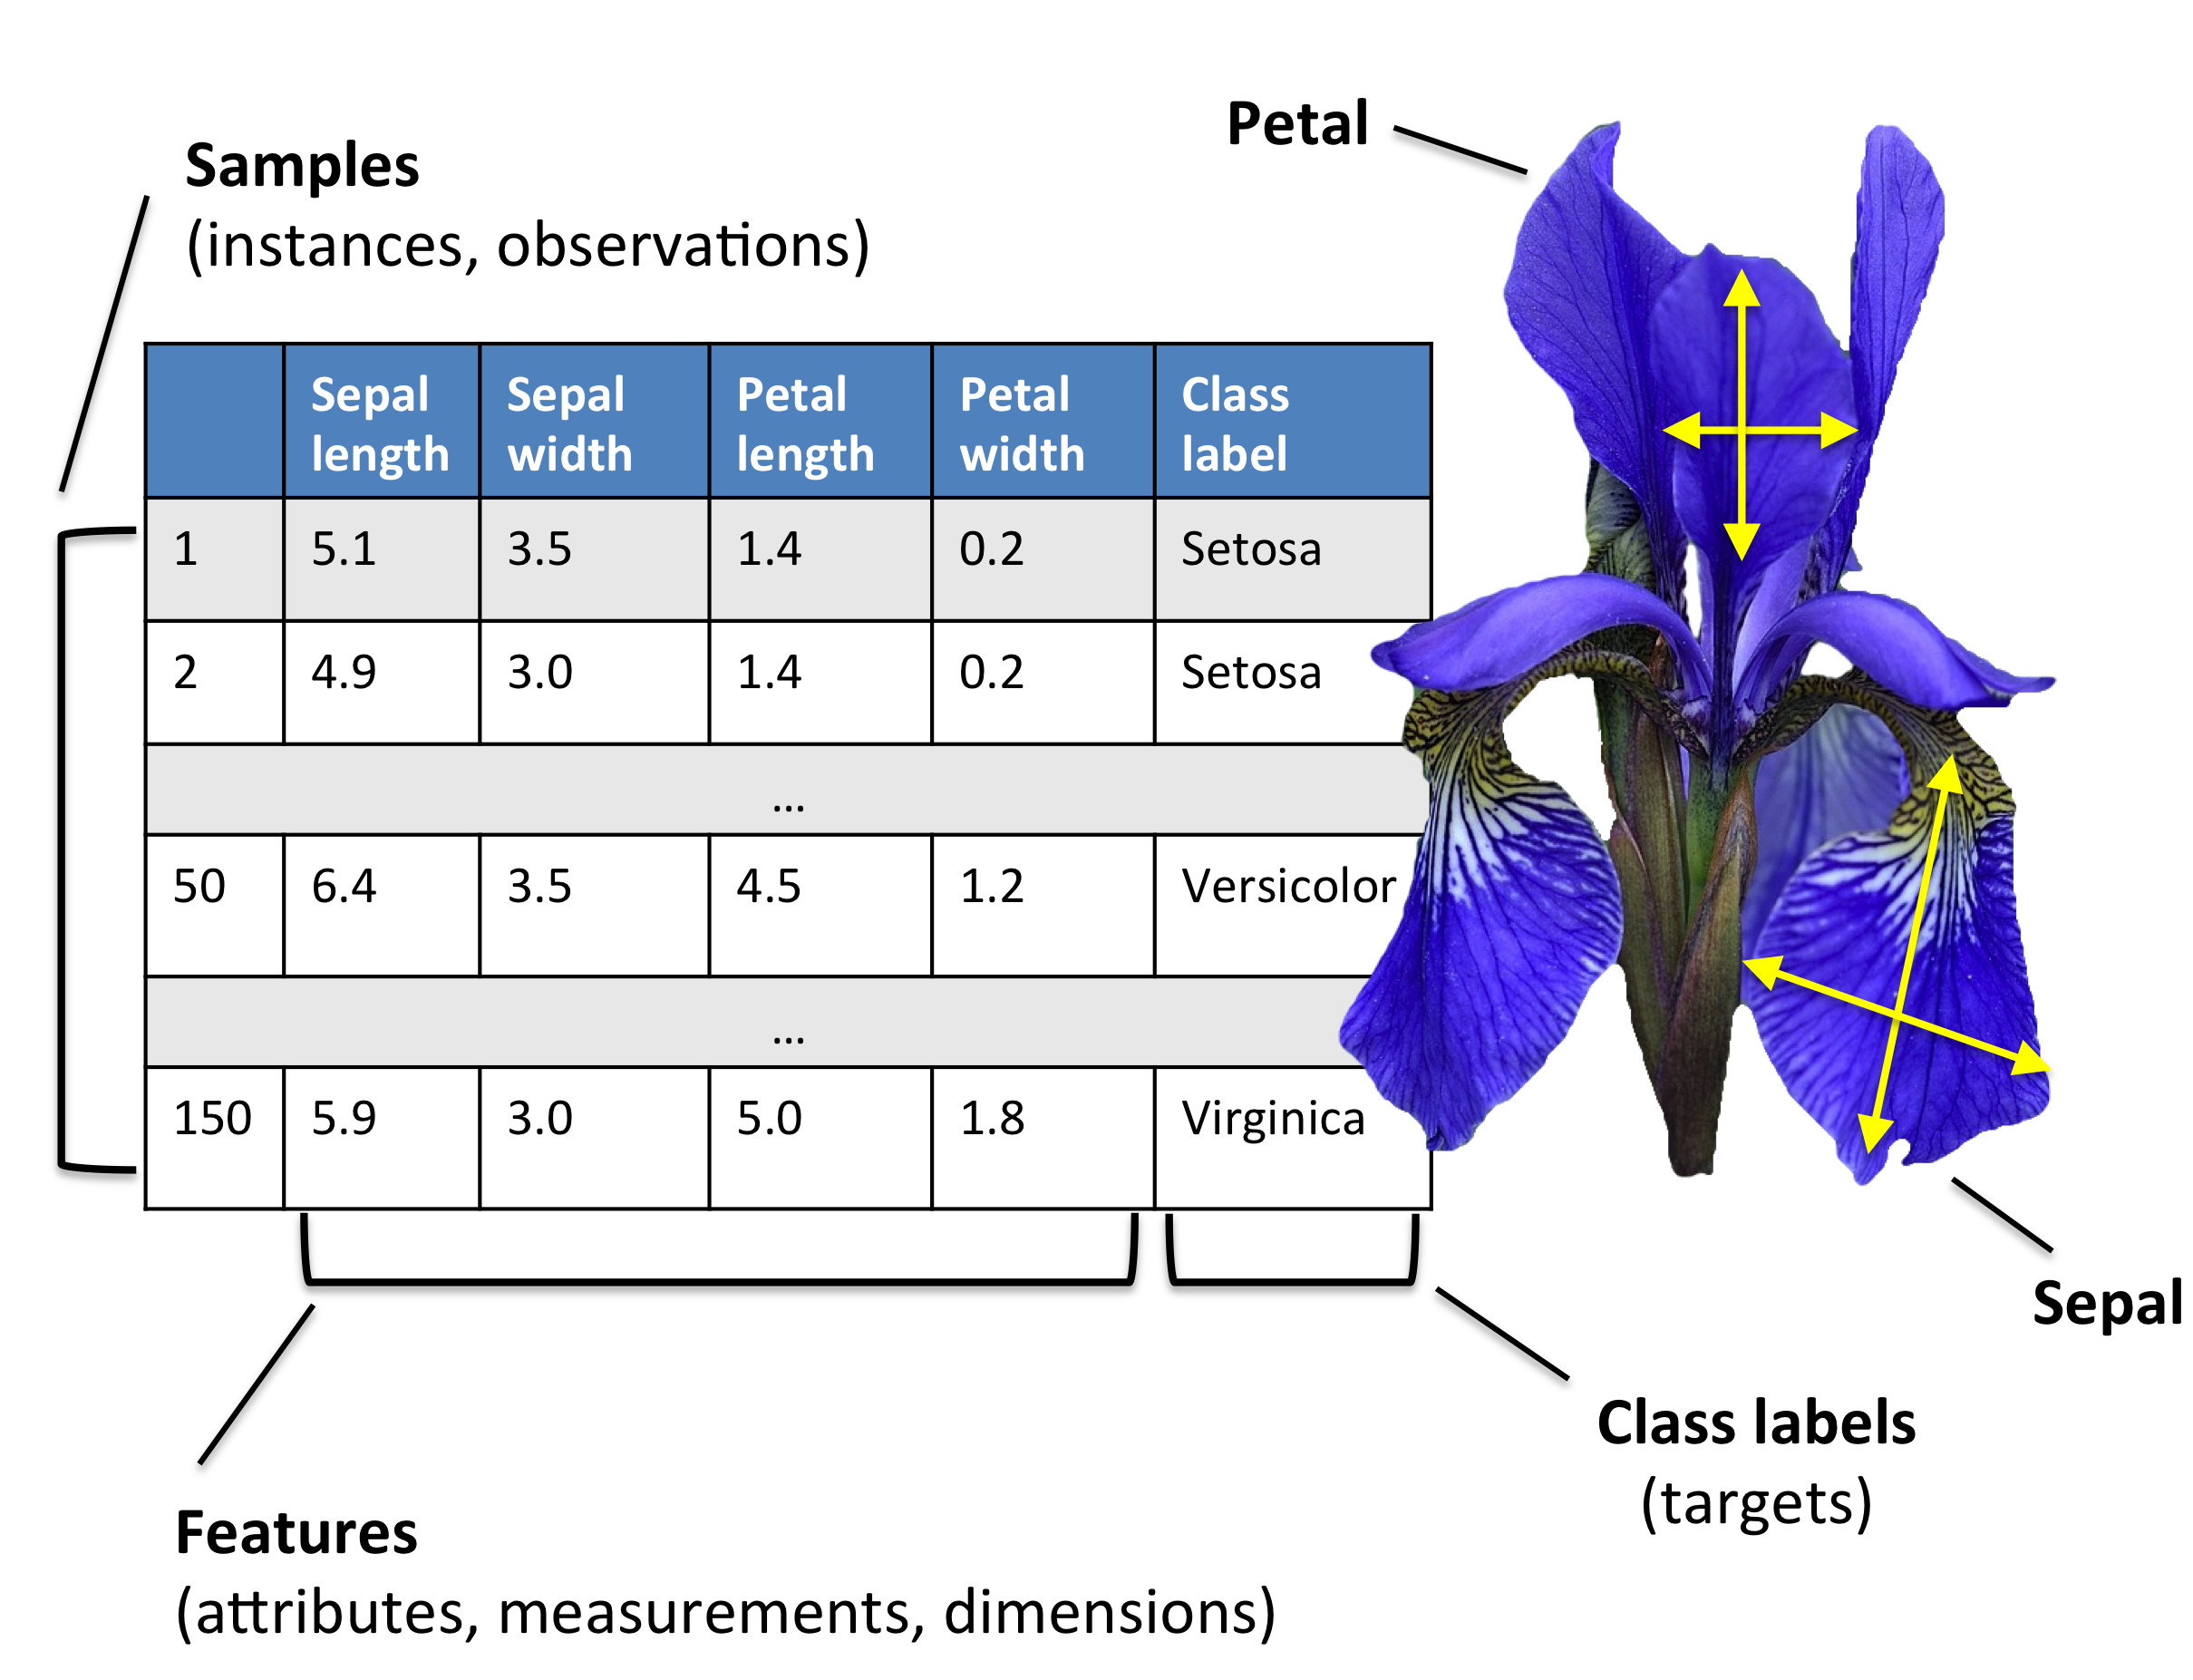
\includegraphics[width=60mm]{img/day01/fig06.png}
        \end{center}
    \end{figure}
    \rightline{\footnotesize ※今回はVirginicaをないものとして扱う。}
    % ※ここでは\(i\)番目のサンプルを\(x^{(i)}\)、\(j\)番目の特徴量を\(x_j\)と表現する。
\end{frame}

\begin{frame}{パーセプトロン}
    人間の神経細胞を模したアルゴリズムで「教師あり学習」の「分類」を行うことができる。 \\
    その表現の対象となった人間の神経細胞では「複数の信号が樹状突起に届き、細胞体に取り込まれる。
    蓄積された信号が特定のしきい値を超えた場合は、軸索によって伝達される」というものである。
    \begin{figure}[b]
        \begin{center}
        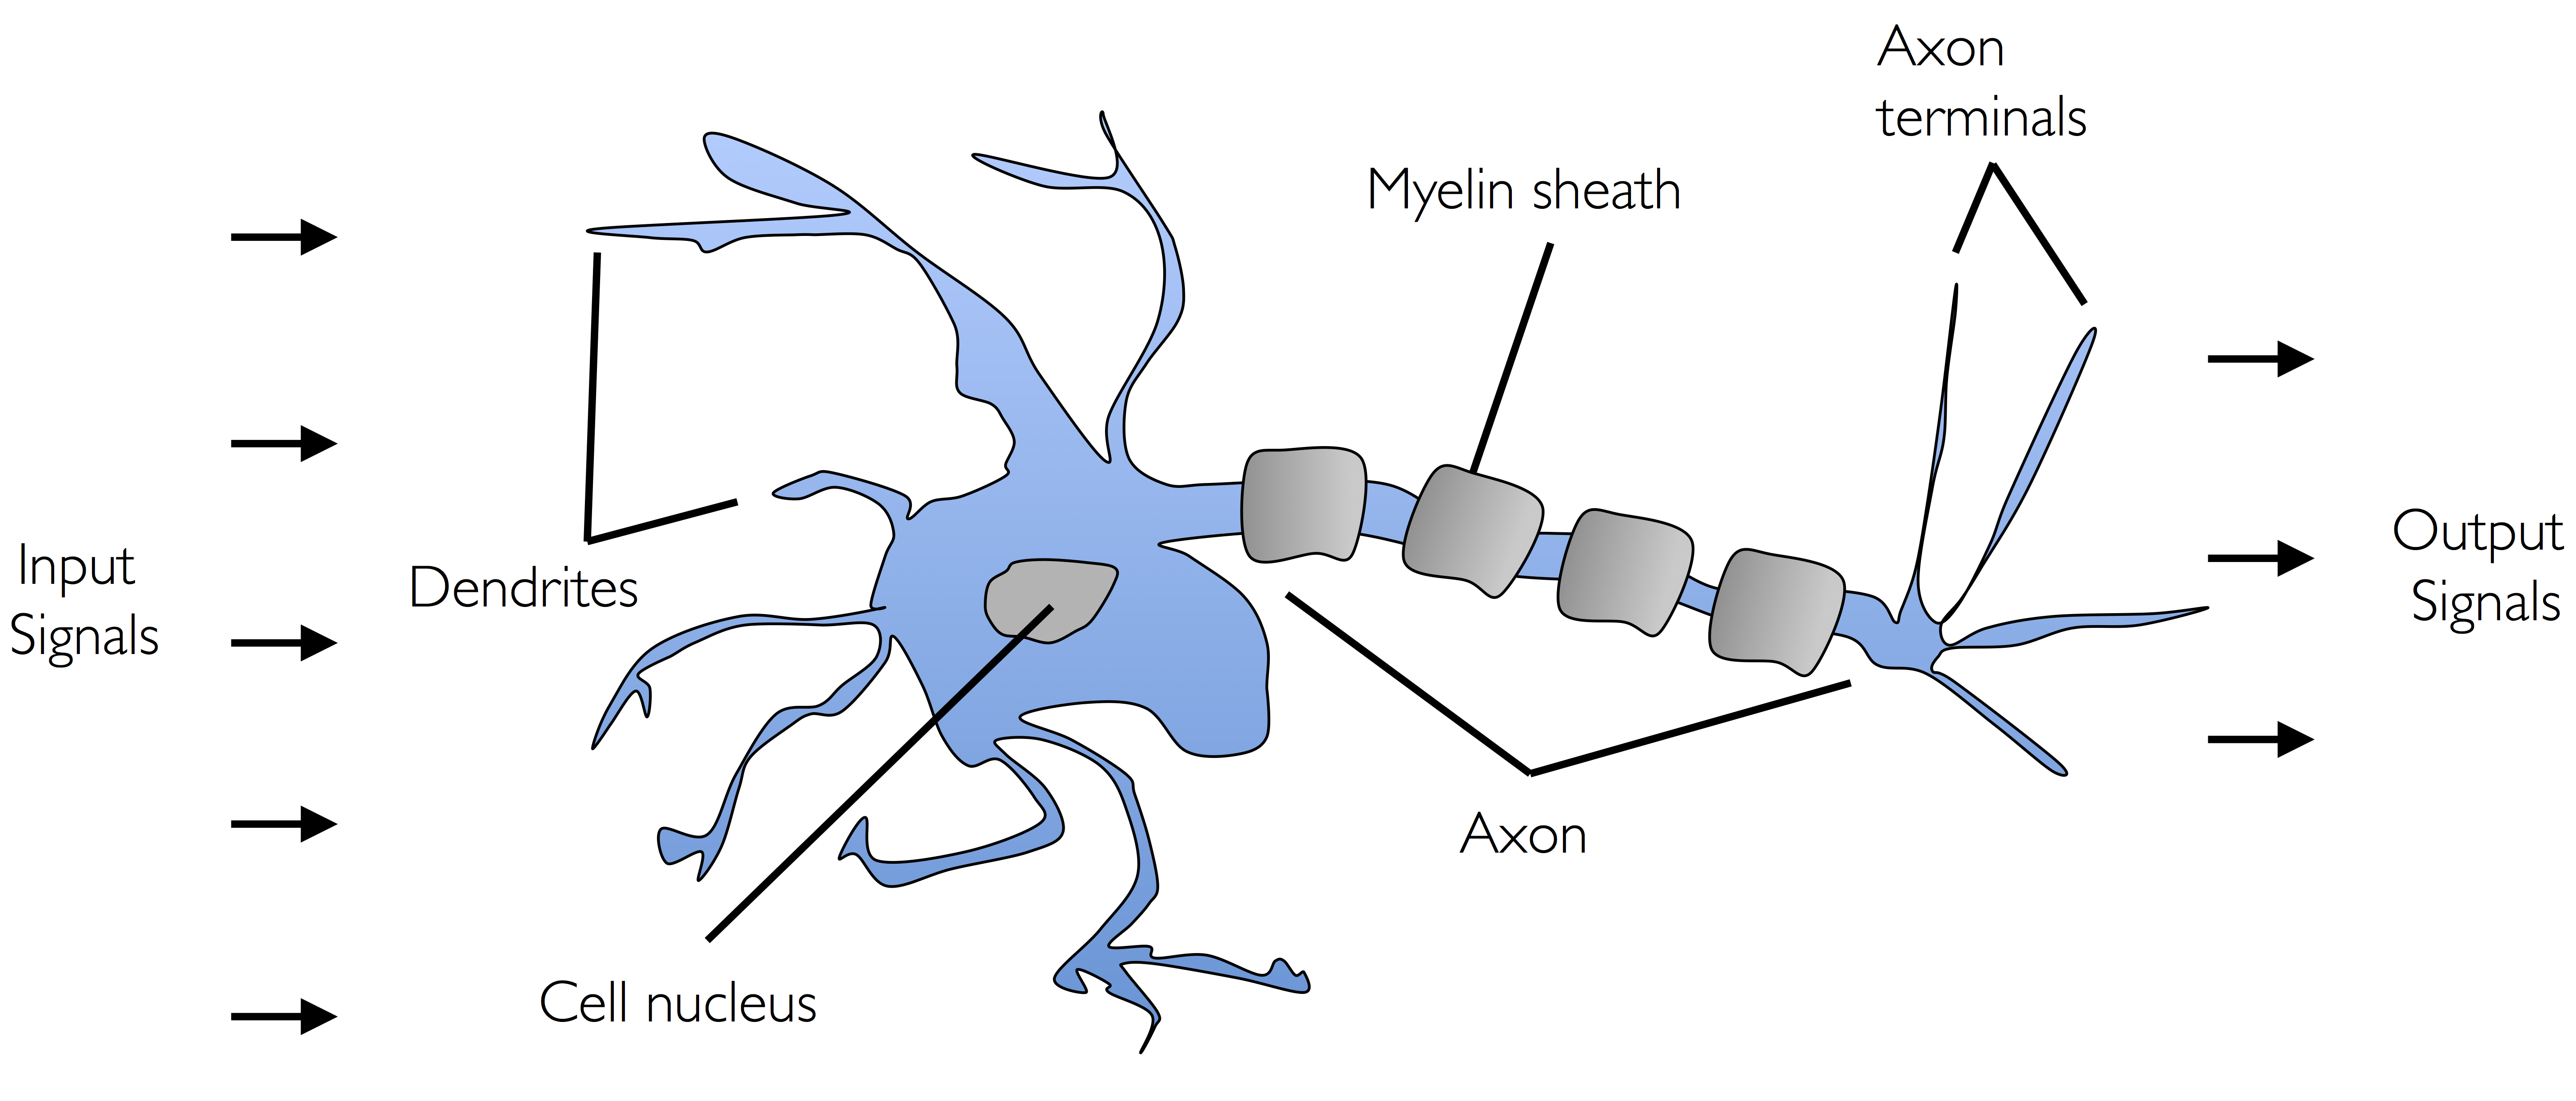
\includegraphics[width=90mm]{img/day01/fig05.png}
        \end{center}
    \end{figure}  
\end{frame}

\begin{frame}{入力}
    信号の入力部分には重み\(w\)と呼ばれるベクトルが存在し、入力の影響力を表している。 \\
    入力値\(\mathbf{x}\)と対応する重みベクトル\boldmath\(w\)の
    線形結合として受け取る。この場合\(z\)は総入力(net input)と呼ばれる。
    \\
    \begin{equation*}
        z = x_1w_1 + x_2w_2 + \cdots  + x_mw_m = \mathbf{w^T}\mathbf{x}
    \end{equation*}
    \\
    \begin{figure}[b]
        \begin{center}
        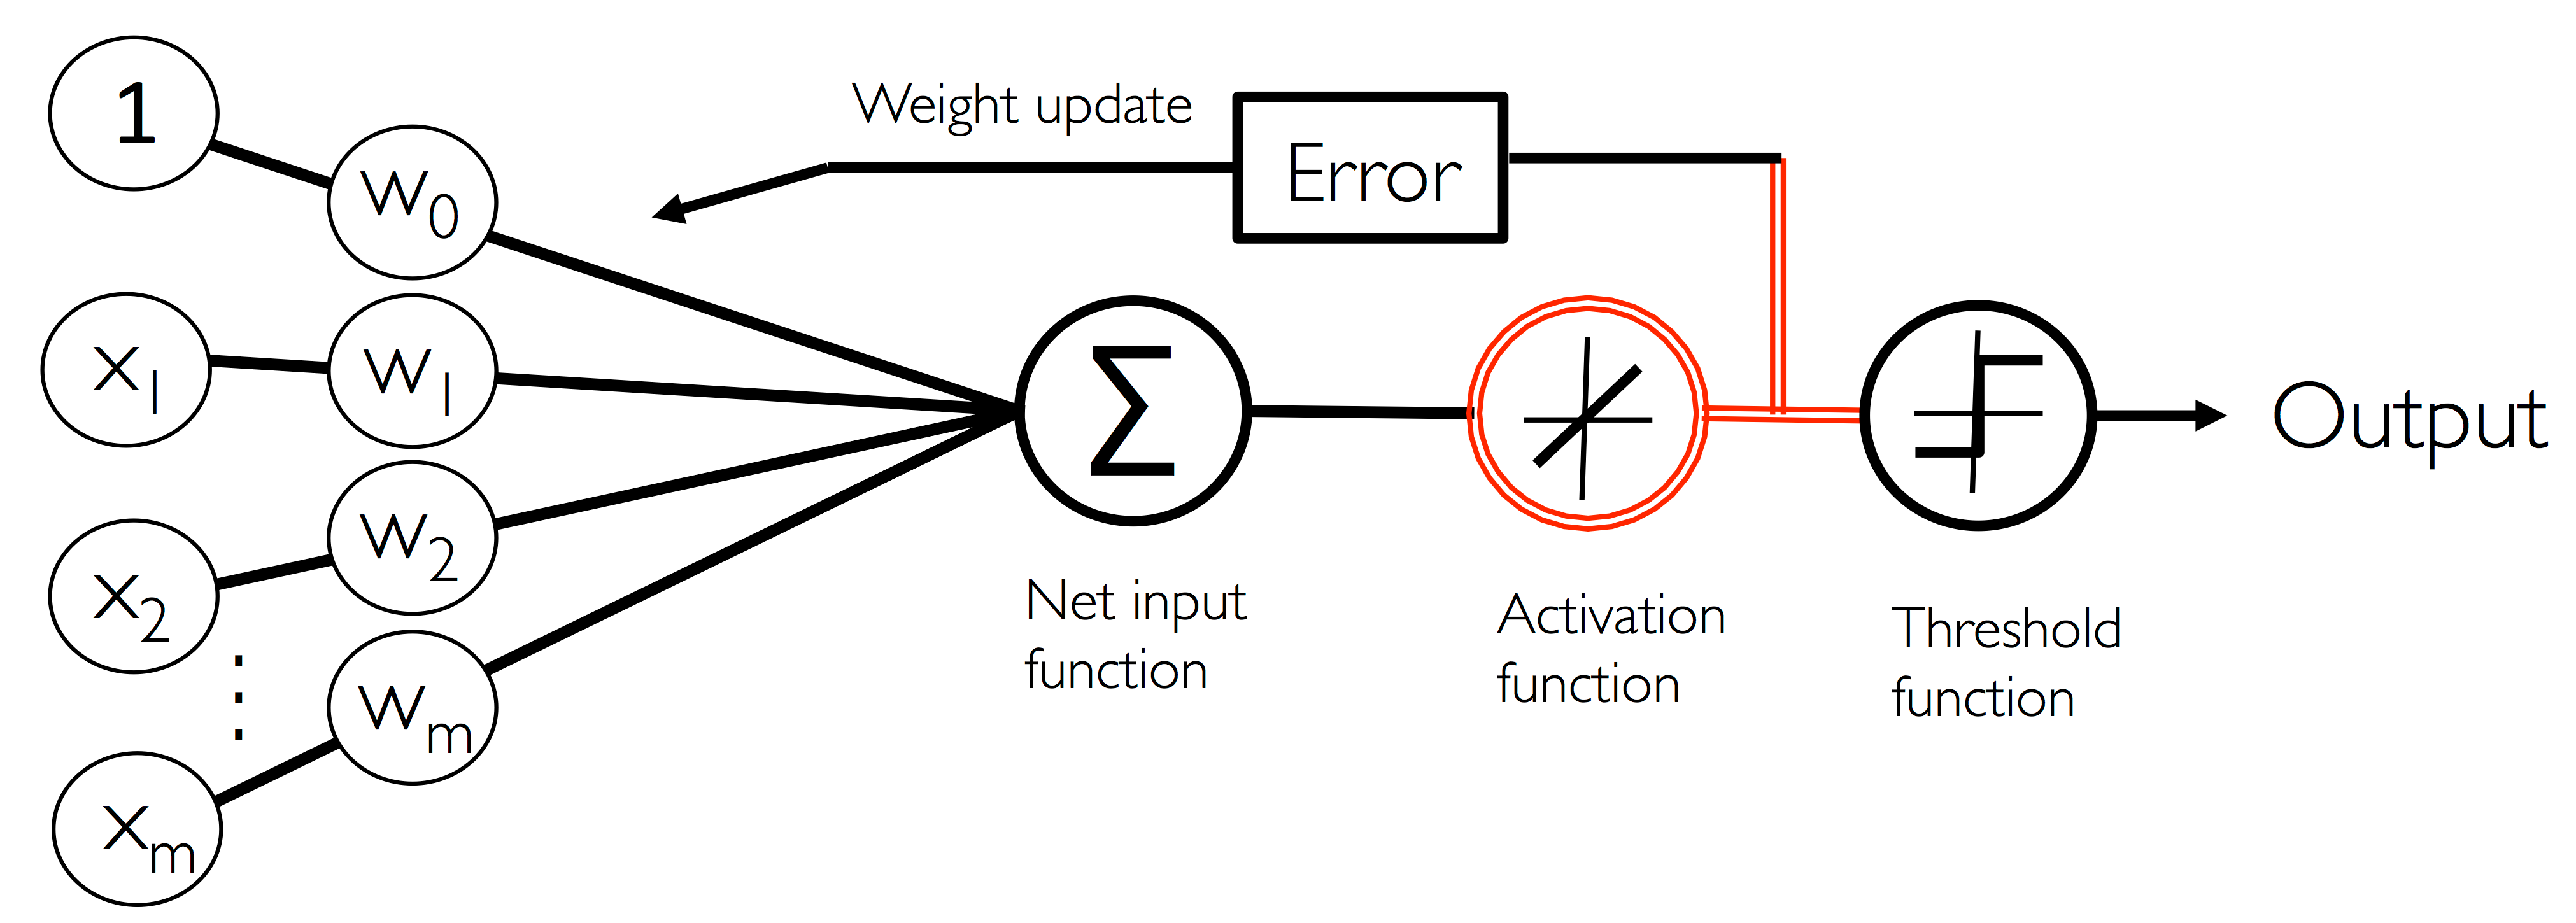
\includegraphics[width=90mm]{img/day01/fig08.png}
        \end{center}
    \end{figure}
\end{frame}

\begin{frame}{決定関数}
    入力データ\(\mathbf(x)\)に対する総入力\(z\)が、指定された閾値\(\theta\)
    よりも大きかった場合に1のクラスを予測し、それ以外の場合は-1のクラスを予測する。
    決定関数\(\phi(z)\)を定義すると以下のようになる。
    \begin{equation*}
        \phi(z) = 
        \begin{aligned}
            & \left\{ \,
                \begin{aligned}
                    &  1 & \quad &(z \geq \theta) \\
                    & -1 & \quad &(z < \theta)
                \end{aligned}
            \right.
        \end{aligned}
    \end{equation*}
    式を単純にするために、閾値\(\theta\)を左辺へ移項し、0番目の重みを
    \(w_0 = -\theta\)および\(x_0 = 1\)として定義すると次の簡潔な式で
    総入力\(z\)を定義できる。
    \begin{equation*}
        z = x_0w_0 + x_1w_1 + \cdots  + x_mw_m = \mathbf{w^T}\mathbf{x}
    \end{equation*}
    \begin{equation*}
        \phi(z) = 
        \begin{aligned}
            & \left\{ \,
                \begin{aligned}
                    &  1 & \quad &(z \geq 0) \\
                    & -1 & \quad &(z < 0)
                \end{aligned}
            \right.
        \end{aligned}
    \end{equation*}
    \(w_0\)のことをバイアスユニット(bias unit)を呼ぶ。
\end{frame}

\begin{frame}{学習}
    パーセプトロンの学習規則は単純で以下の手順で行われる。
    \begin{enumerate}
        \item 重み\(\textbf{w}\)を0か値の小さい乱数で初期化する。
        \item 訓練データ\(\textbf{x}^{(i)}\)ごとに次の手順を実行する
        \begin{enumerate}
            \item 出力値\(\hat{y}\)を計算する。
            \item より良い\(\hat{y}\)になるように重み\(\textbf{w}\)を更新する。
        \end{enumerate}
    \end{enumerate}
    \vspace{1em}
    ここでの出力値は先に定義した決定関数の出力\(\phi(z)\)の出力である。
    重みベクトル\(\textbf{w}\)の各重み\(\textbf{w}_j\)に対する更新式は以下のようになる。
    \begin{equation*}
        w_j := w_j + \Delta w_j
    \end{equation*}
    実際には損失関数の負の勾配(後述)に学習率\(\nabla J(\textbf{w})\)を掛けたものとして定義される。
    \begin{equation*}
        \Delta \textbf{w} = - \eta \nabla J(\textbf{w})
    \end{equation*}
\end{frame}

\begin{frame}{損失関数}
    学習過程で最適化する指標としての関数である目的関数(objective function)を定義する。\\
    多くの場合、この目的関数は最小化すべき損失関数(loss function)である。 \\
    今回の場合は重みの更新に用いる損失関数\(J\)として、誤差平方和(Sum of Squared Error)を定義する。
    \vspace{1em}
    \begin{equation*}
        J(\textbf{w}) = \frac{1}{2}\sum_{i}^{}(y^{(i)} - \phi(z^{(i)}))^2
    \end{equation*}
    \rightline{\footnotesize ※偏微分係数を簡単にするために\(\frac{1}{2}\)を付けています。}\\
    \vspace{1em}
    利点はこの損失関数の利点は微分可能だということである。 \\
    \(J\)を\(\textbf{w}\)で偏微分することによって勾配(微分係数のベクトル)を得ることができる。
\end{frame}

\begin{frame}{SSE(誤差平方和)の偏微分係数}
    \(j\)番目の重み\(w_j\)に対するSSE(誤差平方和)の偏微分系は以下のように求められる。
    \begin{eqnarray*}
        \frac{\partial J}{\partial w_j} &=& \frac{\partial}{\partial w_j} \frac{1}{2} \sum_{n}^{}(y^{(i)}-\phi(z^{(i)}))^2
        = \frac{1}{2} \frac{\partial}{\partial w_j} \sum_{n}^{}(y^{(i)}-\phi(z^{(i)}))^2 \\
        &=& \frac{1}{2} \sum_{n}^{}2(y^{(i)}-\phi(z^{(i)})) \frac{\partial}{\partial w_j} (y^{(i)}-\phi(z^{(i)})) \\
        &=& \sum_{n}^{}(y^{(i)}-\phi(z^{(i)})) \frac{\partial}{\partial w_j} (y^{(i)}-\sum_{k}^{}(w_kx_{k}^{(i)})) \\
        &=& \sum_{n}^{}(y^{(i)}-\phi(z^{(i)})) \frac{\partial}{\partial w_j} (-x_{j}^{(i)})
        = -\sum_{n}^{}(y^{(i)}-\phi(z^{(i)})) x_{j}^{(i)}
    \end{eqnarray*}
    \begin{equation*}
        \therefore \Delta w_i = - \eta \frac{\partial J}{\partial w_j} = \eta \sum_{n}^{}(y^{(i)}-\phi(z^{(i)})) x_{j}^{(i)}
    \end{equation*}

\end{frame}

\begin{frame}{勾配降下法}
    この損失関数のもう1つの利点は、凸関数であること。\\
    凸関数であるので勾配方向に重みを更新していけば損失関数の大域的最小値にたどり着く。\\
    これによって(損失が少ない=)より良い予測結果のパーセプトロンが出来上がる。 \\
    このアルゴリズムを勾配降下法(gradient descent)と呼ぶ。 \\
    \begin{figure}[b]
        \begin{center}
        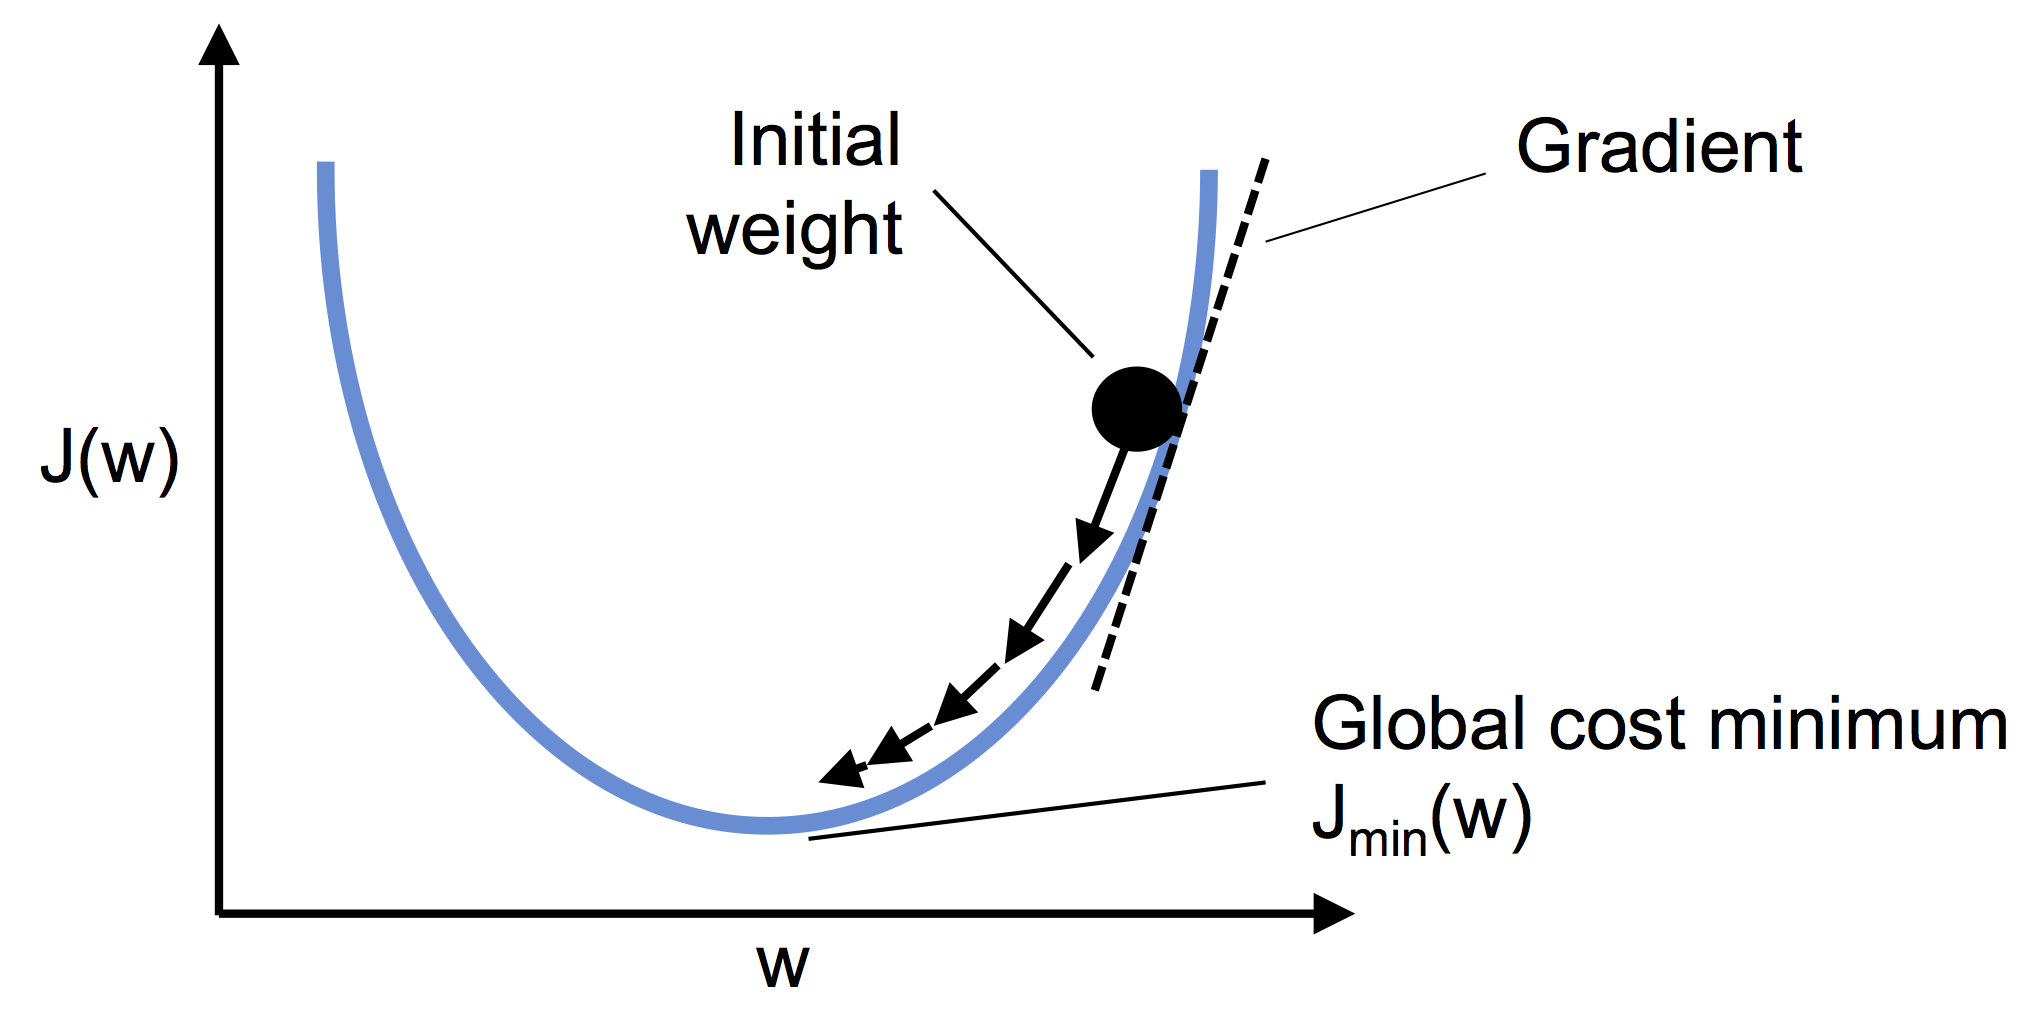
\includegraphics[width=90mm]{img/day01/fig09.png}
        \end{center}
    \end{figure}
\end{frame}

\begin{frame}{学習率}
    学習率を小さく設定しすぎると、少しずつしか重み\(\textbf{w}\)が更新されないので学習が遅くなる。 \\
    一方、学習率が大きすぎると大域的最小値を「超えて」しまうので、逆に誤差が大きくなる。\\
    したがって、適切な学習率を設定することが大切である。
    \begin{figure}[b]
        \begin{center}
        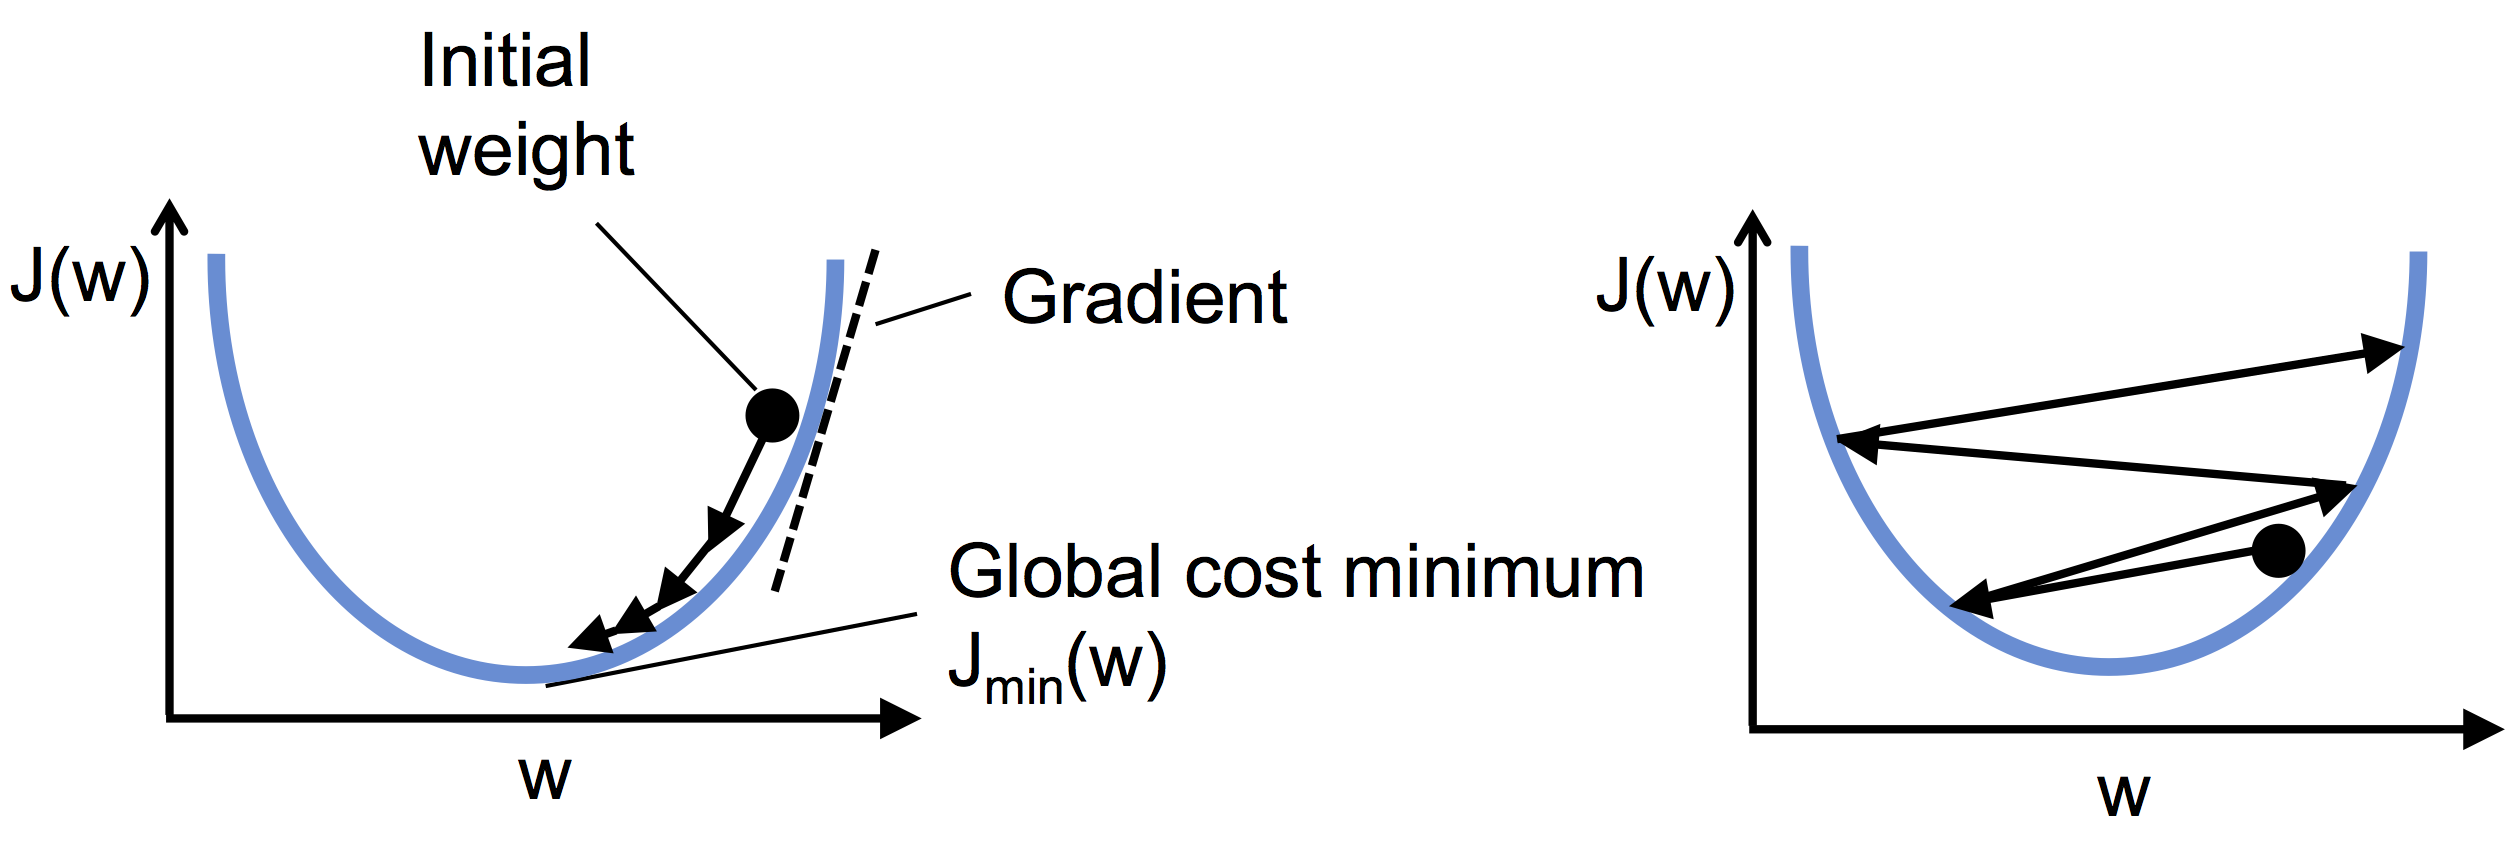
\includegraphics[width=120mm]{img/day01/fig10.png}
        \end{center}
    \end{figure}
\end{frame}

\section{特徴量スケーリング}
\begin{frame}{特徴量スケーリング}
    勾配降下法は特徴量スケーリングの恩恵を受けるアルゴリズムの1つである。 \\
    ここでは標準化(standradization)という手法を用いることで特徴量に順正規分布、ゼロ平均、単位分散
    という特性を持たせて収束を早めることができる。
    \vspace{1em}
    \begin{equation*}
        x_{j}^{'} = \frac{x_j - \bar{x} _j}{\sigma_j}
    \end{equation*}
    \vspace{1em}
    ここで、\(x_j\)はj番目の特徴量の値からなるベクトル、\(\sigma\)は標準偏差である。
\end{frame}

\begin{frame}{特徴量スケーリング}
    標準化が勾配降下法による学習で役に立つ理由の1つは下の図のように
    値の分布を固定することにより損失関数の大域的最小値を見つけ出すための
    ステップ数を少なくできるからである。
    \begin{figure}[b]
        \begin{center}
        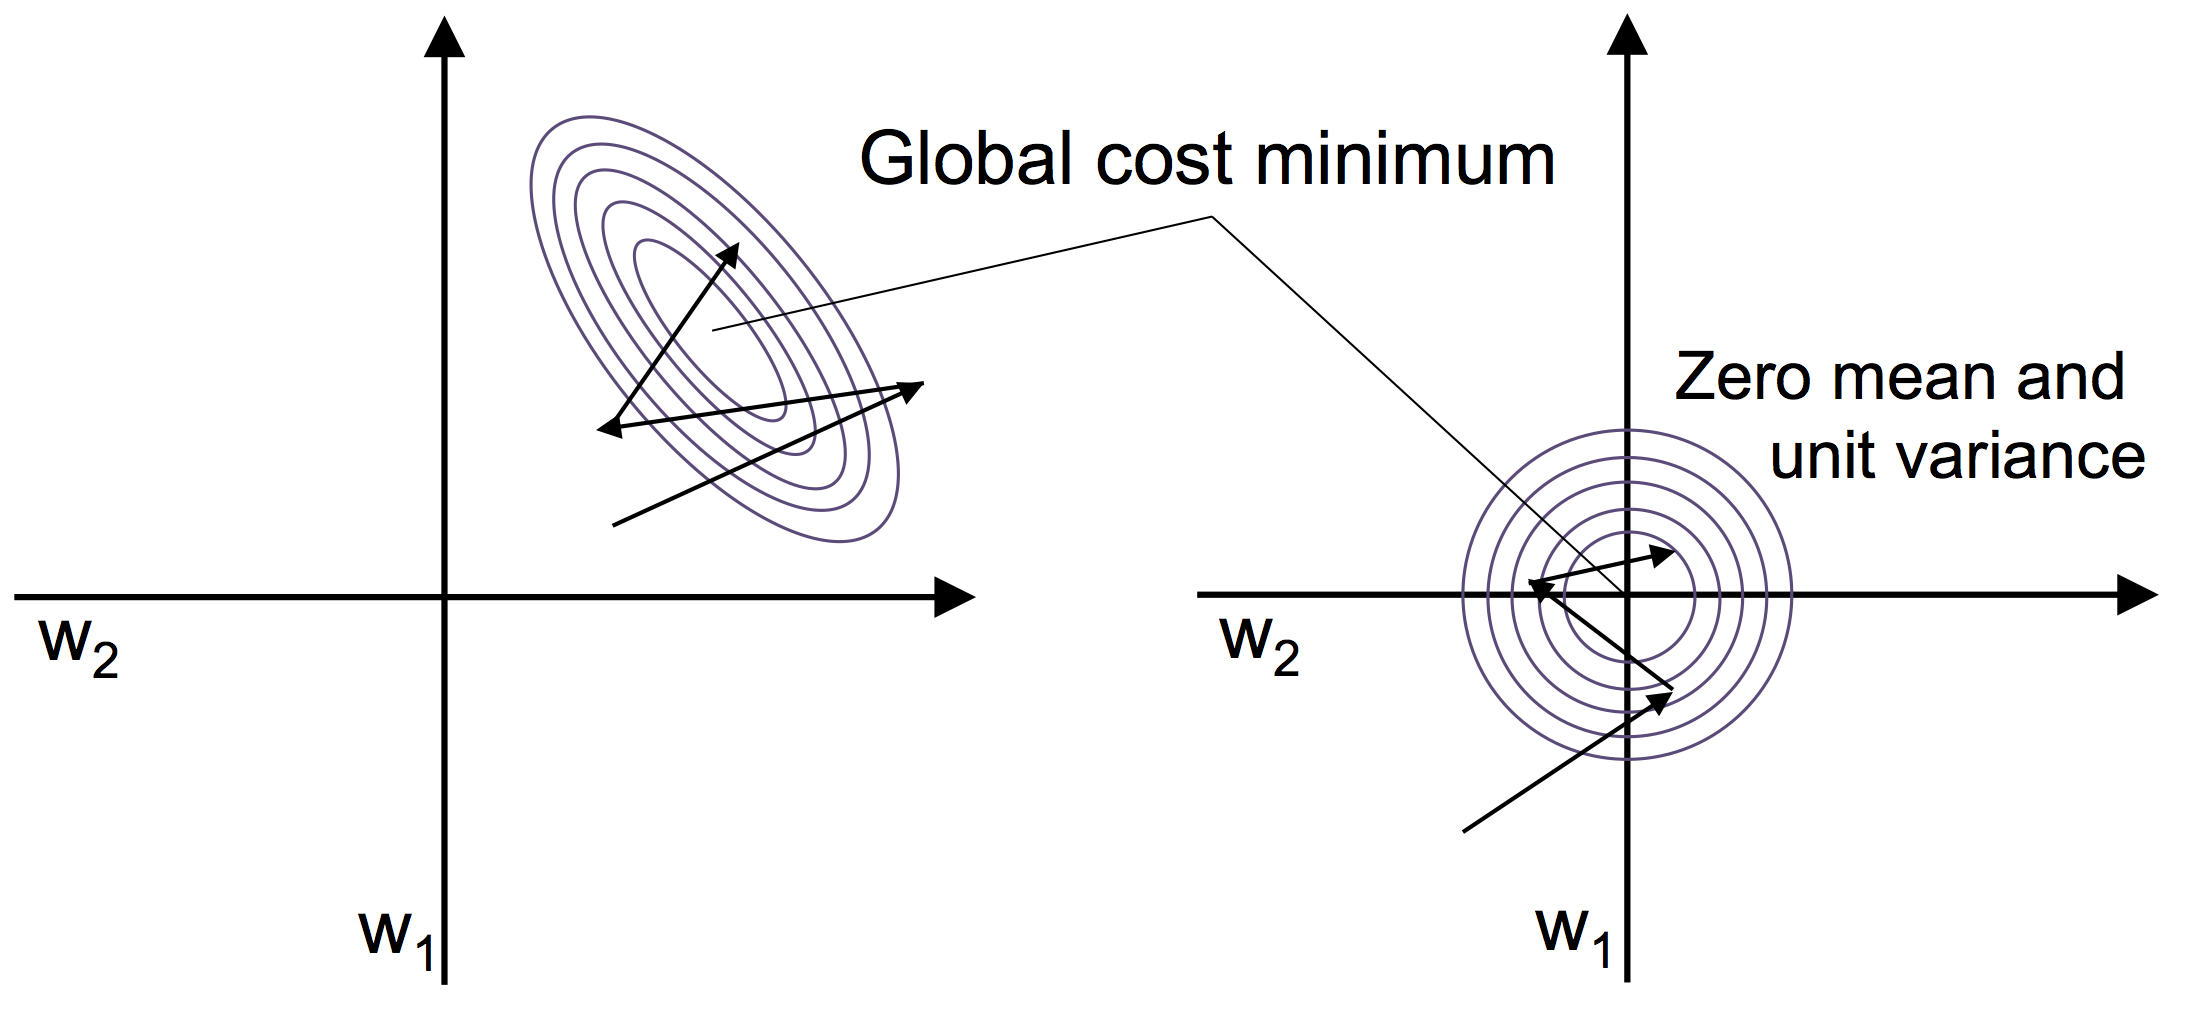
\includegraphics[width=90mm]{img/day01/fig11.png}
        \end{center}
    \end{figure}
\end{frame}

% \section{過学習}
% \begin{frame}{過学習}
%     機械学習の目的は未知のデータに対して正しい予測を行うことである。 \\
%     学習データに対して過剰に適応してしまった場合を過学習(over fitting)と呼ぶ。\\
%     過学習の状態のモデルは学習データに対しては良いスコアを出すが、未知のデータに対してはスコアが出にくい。\\
%     学生に例えると過去問だけを勉強してテスト本番が解けないケース。 \\
%     過学習を防ぐため、学習の際には学習用データとは別にそのモデルが未知のデータに対してどれほどの
%     精度なのかを測定するテストデータを要するのが一般的である。
% \end{frame}

\section{確率的勾配降下法}
\begin{frame}{確率的勾配降下法}
    現在の勾配降下法(最急降下法)はデータ1つごとに重みを更新する必要がある他、
    データをすべてメモリに読み込む必要がある大規模データになってくるOOMを起こす。\\
    このメモリと計算量の問題に対応するために提案された勾配降下法を紹介する。
        \begin{alertblock}{確率的勾配降下法}
            学習データの中からランダムに1セットだけを取り出して損失を計算している。
            すべてのデータをメモリ上に読み込む必要がなく、一度に1セットのデータでしか損失を計算しない。
        \end{alertblock}
        \begin{exampleblock}{ミニバッチ勾配降下法}
            学習データの中からランダムに\(B\)個のデータを取り出して、損失を計算する。\\
            ディープラーニングでよく利用されるアルゴリズム。\(B\)は batch size.
        \end{exampleblock}
\end{frame}

\end{document}